\documentclass[preprint]{sigplanconf}
\usepackage{amssymb}
\usepackage{amsthm}
\usepackage{graphicx}
\usepackage{amsmath}
\usepackage{mathptmx}
\usepackage{mathtools}
\usepackage{stmaryrd}
\usepackage{hyperref}
\usepackage{alltt}
\usepackage{url}
\usepackage{float}
\usepackage{tikz}
\usepackage{pgfplots}
\usepackage{style/code}
\usepackage{style/proof}
\usepackage{style/utils}
\usepackage{style/judgements}

% -----------------------------------------------------------------------------
\begin{document}

% \exclusivelicense
% \conferenceinfo{}{}
% \copyrightyear{2015}
% \copyrightdata{}
\doi{}
% \pagenumbering{gobble} 

\title{Icicle: write once, run once}

\authorinfo{
  Amos Robinson$^{\alpha \beta}$
  \and Ben Lippmeier$^{\beta \gamma}$
}{
  \vspace{5pt}
  \shortstack{
    $^\alpha$Ambiata      \\
    Grow with data          \\[2pt]
    \textsf{amos.robinson@ambiata.com}
  }
  \shortstack{
    $^\beta$UNSW Australia\\
    \\[2pt]
    ~~~~\textsf{amosr,benl@cse.unsw.edu.au}
  }
  \shortstack{
    $^\gamma$Vertigo Technology \\
    \\[2pt]
    ~~\textsf{benl@vergo.co}
  }
}

\maketitle
\makeatactive

\begin{abstract}
We present a pure query language, Icicle, which statically guarantees that multiple queries over the same input data set will be fused. We include a modal type system that guarantees these fused results will be evaluated with a single pass over the input data. Icicle queries are compiled via a fold-based intermediate language to efficient C code. We present production benchmarks demonstrating significant speedup over existing queries written in R, as well as the widely used Unix tools \texttt{grep} and \texttt{wc}.

% When querying a large amount of data, simply iterating over the data may take hours. If multiple queries are to be performed, it is important that work is not duplicated. Queries that can be performed together must be performed in the same iteration. We introduce a simple streaming language for computing queries in a single-pass over the data. With type and other restrictions we guarantee fusion between queries on the same input table, before extracting efficient C code.
\end{abstract}


\category
	{D.3.4}
	{Programming Languages}
	{Processors---Compilers; Optimization}

\terms
	Languages, Performance

\keywords
	Arrays; Fusion

%!TEX root = ../Main.tex
\section{Introduction}
\label{s:Introduction}

Suppose we have two input streams of numeric identifiers, and wish to perform some analysis on these identifiers. The identifiers from both streams arrive sorted, but may include duplicates. We wish to produce an output stream of unique identifiers from the first input stream, as well as produce the unique union of identifiers from both streams. Can we perform both of these tasks at once, without needing to read through the stream data multiple times, and without needing unbounded buffering? Here is how we might write the source code, where @S@ is for @S@-tream.
\begin{code}
  uniquesUnion : S Nat -> S Nat -> (S Nat, S Nat)
  uniquesUnion sIn1 sIn2
   = let  sUnique = group sIn1
          sMerged = merge sIn1 sIn2
          sUnion  = group sMerged
     in   (sUnique, sUnion)
\end{code}

In this implementation the @group@ operator filters out consecutive duplicates, while @merge@ combines two sorted streams so that the output remains sorted. This example has a few interesting properties. Firstly, the data-access pattern of @merge@ is \emph{value-dependent}, meaning that the order in which this operator pulls values from @sIn1@ and @sIn2@ depends on the values themselves. If all the values from @sIn1@ are smaller than the values in @sIn2@, then @merge@ will pull all values from @sIn1@ before pulling the rest from @sIn2@, and vice versa. Secondly, although @sIn1@ occurs twice in the program, at runtime we only want to handle the elements of each stream once. To achieve this, the compiled program must coordinate between the two uses of @sIn1@, so that values are only read when both the @group@ and @merge@ operators are ready to receive a new value. Finally, as the stream length is assumed to be unbounded, we cannot buffer an arbitrary number of elements read from either stream, or risk running out of local storage space.

For an implementation which does \emph{not} use stream fusion, we might implement each of the operators as a separate concurrent process, and send each identifier value using an intra-process communication mechanism. Developing such an implementation could be easy or hard, depending on what language features are available for concurrency. However, worrying about the \emph{performance tuning} of such a system, such as whether we need back-pressure, or how to chunk the stream data to reduce the amount of communication overhead, is invariably a headache. 

We might instead define some sort of uniform interface for data sources, with a single `pull' function that provides the next value in each stream. Each operator could be given this interface, so that the next value from each result stream is computed on demand. This is approach is commonly taken with implementations of physical operators in data base systems. However, this `pull only' model does not support operators with multiple outputs, such as our derived @uniquesUnion@ operator, at least not without unbounded buffering. Suppose a consumer pulls many elements from the result @sUnique@ stream. The implementation needs to pull the corresponding source elements from @sIn1@ \emph{as well} as buffering an arbitrary number of matching elements from @sIn2@. It needs to buffer an aribrary number of elements from @sIn2@ because there is no guarantee of when a consumer will also pull from the @sUnion@ result stream. Once that happens the elements from @sIn2@ no longer need to be retained, but not before.

Instead, for a single threaded program, we want to perform \emph{stream fusion}, which takes the dataflow network and produces a simple sequential loop that gets the job done without requiring extra process-control abstractions and without requiring unbounded buffering. Sadly, existing stream fusion transformations cannot handle our example. As observed by \citet{kay2009you}, both pull-based and push-based fusion have fundamental limitations. Pull-based systems such as short cut stream fusion~\cite{coutts2007stream} cannot handle cases where a particular stream or intermediate result is used by multiple consumers. We refer to this situation as a \mbox{\emph{split} --- in the} dataflow network the flow from input stream @sIn1@ is split into both the @group@ and @merge@ consumers. 

% Leave this to related work. We've already mentioned a canonical pull-based system.
% Recent work on stream fusion by \citet{kiselyov2016stream} uses staged computation to ensure all combinators are inlined, but for splits this causes excessive inlining which duplicates work, due to values of the source arrays being read multiple times.

Push-based systems such as foldr/build fusion~\cite{gill1993short} also cannot fuse our example because they do not support operators with multiple inputs. We refer to such a situation as a \emph{join} --- in our example the @merge@ operator expresses a join in the data-flow graph. Some systems support both pull and push: data flow inspired array fusion~\cite{lippmeier2013data} allows both splits and joins but only for a limited, predefined set of operators. More recent work on polarized data flow fusion~\cite{lippmeier2016polarized} \emph{is} able to fuse our example, but requires the program to be rewritten to use explicitly polarized stream types. 

% The mechanism that combines the implementations of both operators, to yield efficient imperative code also depends on the general purpose compiler optimisations implemented by GHC, and it can be difficult to tell if these have ``worked'' without inspecting the intermediate representations of the compiler.

Synchronous dataflow languages such as Lucy-n~\cite{mandel2010lucy} reject value-dependent operators such as @merge@, while general dataflow languages fall back on less performant dynamic scheduling for these cases \cite{bouakaz2013real}. The polyhedral array fusion model~\cite{feautrier2011polyhedron} is used for loop transformations in imperative programs, but operates at a much lower level. The polyhedral model is based around affine loops, which makes it difficult to support filter-like operators such as @group@ and @merge@.

In our new system we still view the program as a concurrent process network. Each operator is a separate process, and the stream data flows through communication channels between the processes. Each operator is expressed as a restricted, sequential imperative program with commands that include both @pull@ for reading from an input stream and @push@ for writing to an output stream. The fusion transform takes the concurrent process network and \emph{sequentializes} it into a single process by choosing a particular evaluation order that requires no unbounded intermediate buffers. When the fusion transformation succeeds we know it has worked. There is no need to inspect intermediate representations of the compiler to debug poor performance, which is a common problem in systems based on general purpose program transformations \cite{lippmeier2012:guiding}.

In summary, we make the following contributions:
\begin{itemize}
\item a process calculus for encoding infinite streaming programs (\S\ref{s:Processes});
\item an algorithm for fusing these processes, the first to support arbitrary splits and joins (\S\ref{s:Fusion});
\item numerical results that demonstrate that the algorithm is well behaved when the number of fused processes is large. The size of the fused result program is not excessive. \TODO{Ref}
\item a formalization and proof of soundness for the core fusion algorithm in Coq (\S\ref{s:Proofs});
\end{itemize}

Our fusion transformation for infinite stream programs could also serve as the basis for an \emph{array} fusion system, using a natural extension to finite streams. We discuss this extension in \S\ref{s:Finite}.

% TODO: We can't make the appendix a contribution because the reviewers are not required to read appendices.
% \item and show our processes are general enough for many combinators, including segmented operations (\S\ref{s:Combinators}).

% \ben{Add a few more sentences on related work. Explain how this work extends the old flow fusion paper. It is not short-cut fusion like Oleg's recent work. We are not in the same space as Fortran style array fusion transformations like polyhedral}

% BL: describe this later.
% Furthermore, the data-flow fusion system of~\cite{lippmeier2013data} only deals with a fixed set of baked-in combinators. 

% BL: Shift the detailed description into a later section.
% The example above has three combinators, so the process network has three processes.
% The two @writeFile@s outputs are treated as sinks that values can be pushed to at any time, and are not converted to processes.
% During code generation, any output values from the @uniques@ and @union@ streams are sent to the corresponding @writeFile@ sink, but we do not address code generation in this paper.

% The process for @uniques@ is defined by the @group@ combinator, and can be thought of as an imperative loop: first it reads from its input stream @file1@ and stores that in a local variable.
% It also keeps track of the last pulled value, and compares that against the newly read value.
% If they are different, it pushes the new value to its output stream @uniques@.
% In either case, it updates the last pulled value and loops back to the start to pull from @file1@ again.

% The process for @merged@ is defined by the @merge@ combinator, which starts by reading from both @file1@ and @file2@ and storing these in local variables.
% It then compares its two values to see which is the smaller.
% If the value from @file1@ is smaller, it pushes that value and pulls a new value from @file1@, otherwise it pushes the value from @file2@ and pulls from @file2@.
% This is performed in a loop.

% We fuse these two processes by interleaving the two such that the shared input @file1@ is only pulled from when both processes agree.
% The new process pulls from @file1@, which is copied to the variables for both processes.
% The @uniques@ process now has all it needs to execute, so it checks the value against the last pulled value, pushes if necessary, and goes back to try to pull from @file1@ again.
% At this stage the @merged@ process still has a value from @file1@ that it has pulled but not used, so @uniques@ cannot pull from @file1@ again.
% We now let @merged@ run, pulling from @file2@ and checking which is smaller.
% If the value from @file1@ is smaller, the value is emitted and @merged@ wishes to pull a new value from @file1@.
% Both processes now agree on pulling from @file1@ again, so the new value is pulled and @uniques@ can run again.
% Otherwise if the value from @file1@ is not smaller, the value from @file2@ is emitted and @merged@ pulls from @file2@ with no coordination required.

% If we wish to ensure that each value is only read from the file once, we must coordinate between the two use sites: when @uniques@ requires a new value it must ensure that @union@ is ready to receive a new value, and vice versa. Note that we cannot just execute @uniques@ while storing the read values in a buffer, as this may require more memory than is available.
% In order to fuse this example, we require both pull \emph{and} push streams.
% The input streams must be pull streams since the order values are required is determined by the @merge@ combinator.
% For the same reason, the outputs sent to each @writeFile@ must be push streams.

% Fusion for array programs is important for removing intermediate arrays, reducing memory traffic and reducing allocations.
% However, when dealing with data too large to fit in memory such as tables on disk, removing intermediate arrays becomes essential rather than just desirable.
% Attempting to create an intermediate array of such amounts of data would lead to thrashing and swapping to disk, or perhaps even running out of swap.
% For these situations, some sort of assurance of total fusion is required: either the program can be fused with no intermediate arrays or unbounded buffers, or it will not compile at all.


% Fusion eliminates intermediate array buffers and converts pipelines of array combinators into low-level iteration based loop code. Different fusion systems can handle 

% When comparing fusion systems, three important criteria to consider are: whether the system supports splits, where a stream is used multiple times; whether it supports joins, where a combinator has multiple inputs; and whether arbitrary combinators such as @merge@ and segmented appends can be encoded. Existing fusion systems support one or two of these, but not three. We present a fusion system based on process calculus that supports all three: splits, joins and arbitrary combinators.

% Our system has been formalised in Coq where we have proved soundness of the fusion algorithm. It is expressive enough to encode a wide range of combinators including operations on segmented arrays.

% \amos{``Arbitrary combinators'' is not quite true. How can we distinguish combinators we support from 2013 data flow fusion paper? Perhaps by mentioning value-dependent input / access patterns.}

% Leave this to the description of the algorithm, not the abstract.
% We encode each combinator as a separate process with any number of input and output channels. Each process is sequential but multiple processes can be executed concurrently. We give a concurrent execution semantics for multiple processes, but these are used only as a specification for how the fused program must behave. The fused program itself is sequential and can easily be converted to simple imperative code.

% Our fusion algorithm takes two concurrently executable processes and creates a sequential interleaving of the two such that they execute with no unbounded buffers.
% If fusion would require unbounded buffers (or the fusion algorithm wrongly infers that it would) then fusion fails.
% If fusion fails, the user can be presented with an error message telling them which combinators could not be fused.
% For scenarios where fusion is required, this is a great advantage over fragile shortcut fusion systems.

% BL: leave the apologies to the conclusion.
% The version presented here deals with infinite streams, and we informally describe the extensions required to support finite streams.

% BL: leave this to the main intro.
% optimising high-level array and streaming computations, as it reduces memory traffic and intermediate arrays. The benefits of removing intermediate arrays are even more important as data sizes approach the size of memory.

%!TEX root = ../Main.tex
\section{Icicle Source}
\label{s:Source}

In this section we describe the grammar and evaluation semantics of the Icicle language.

Icicle queries execute over a single table, which must at least contain an entity identifier and a date.
Each query implicitly groups the data by entity and sorts it by date, before iterating through the data and computing some aggregate.
We define the stocks table as follows, leaving out the company code (entity identifier) and date.

\begin{tabbing}
MM \= MM \= MMMMMMMMMMM \= \kill
$@table@~\mi{stocks}$    \\
$\{$ \> $\mi{open}$ \> $:~\NN$ \\
$~,$ \> $\mi{close}$ \> $:~\NN$ \\
$\}$
\end{tabbing}

This defines the columns as natural numbers, and allows them to be referred to by name.
In the definitions and queries below, any reference to these names means the column itself, with the entire data for a given entity.
This is annotated with the mode @Element@, meaning that it exists for every element of the input.

We now define some useful functions and other definitions that can be used in the queries themselves.

First we define a function to compute the sum of some input data.
While traditionally sum would take just an input stream of numbers, we separate this into two distinct parameters.
The first parameter is the clock for the input stream, which defines the parts of the input stream to sample.
This can be thought of as a stream of boolean flags, where true denotes that the input stream should be sampled at this time.
The second parameter is the actual value to sample at the clock.
In Icicle this has type $\Elm{\NN}$, meaning it is available as a number at any part of the stream.

By separating the clock from the element values, we guarantee that any references to elements denote the same point in the stream, and can always be used together.
For example, computing the difference between the two fields above ($\mi{open} - \mi{close}$) refers to the open and close fields at the same point.
The clock is used when performing a fold, and determine at which points to sample the elements and update the accumulator.
This is in constrast to traditional streaming dataflow languages, where the element data and the clock are intertwined.
This requires clock analysis\CITE to tell whether two element streams can be used together with a bounded buffer.

We denote clocks in brackets as they are a different universe to normal expressions.
\begin{tabbing}
MM \= MM \= MMMMMMMMMMM \= \kill
@function@ 
$\mi{sum}[c]~v$    \\
\> $=$  \> $@fold@[c]~s~=~0~@then@~s~+~v$ \\
\> @in@ \> $s$. \\
\end{tabbing}

The result of $\mi{sum}$ above has type $\Agg{\NN}$.
Aggregate types denote that their value is only available after the entire input stream has been seen.
By restricting the bodies of folds to be element types, and their output to be aggregate types, it means no reference to the result of folds can be made in the body of a fold.

We can define a query that computes the sum of each company's open prices.
Query definitions are similar to function definitions, except they only take one argument: the clock describing all available input.
They also must return aggregates, as an element query could be unbounded in size.
\begin{tabbing}
MM \= MM \= MMMMMMMMMMM \= \kill
@query@ 
$\mi{opensum}[c]$    \\
\> $=$  \> $\mi{sum}[c]~\mi{open}$. \\
\end{tabbing}

We can run $\mi{opensum}$ over some example data.
This example data has the company code and date for each entry, as well as the stock's open and close prices.
Note that the sum only becomes available at the end of each entity, and only applies to a particular entity's elements.

\begin{code}
CODE, OPEN, CLOSE, DATE,        OPENSUM
ABC,    10,    12, 2015-01-01,       10
IAG,    11,    12, 2015-01-01
IAG,    12,    10, 2015-01-02,       23
\end{code}


Next, we can define functions $\mi{count}$ and $\mi{mean}$ in terms of $\mi{sum}$.
Count passes the argument $1$ to sum, and this is interpreted as an element containing all ones.
The input clocks are passed along as-is.
\begin{tabbing}
MM \= MM \= MMMMMMMMMMM \= \kill
@function@ 
$\mi{count}[c]$                                     \\
 \> $=$  \> $\mi{sum}[c]~1$.                           \\
                                                    \\
@function@ 
$\mi{mean}[c]~v$                                       \\
 \> $=$  \> $\mi{sum}[c]~v~/~\mi{count}[c]$.              \\
\end{tabbing}

Clocks can be reduced to filter out certain elements using @where@.
In this query, we use @where@ to count the number of days where the close price is higher than the open price.
\begin{tabbing}
MM \= MM \= MMMMMMMMMMM \= \kill
@query@ 
$\mi{gap}[c]$                                        \\
 \> $=$  \> $\mi{count}[c~@where@~\mi{close}~>~\mi{open}]$.       \\
\end{tabbing}

In the example below we have shown the result of the element expression $\mi{close}~>~\mi{open}$ for clarity only; this is not included in the output of the $\mi{gap}$ query.
\begin{code}
CODE, OPEN, CLOSE, CLOSE > OPEN, GAP
ABC,    10,    12,            T,   1
IAG,    11,    12,            T
IAG,    12,    10,            F,   1
\end{code}

\TODO{Mention resumables and bubblegum?}

\TODO{Talk about scan}

We formally define the grammar of the language in figure~\ref{fig:source:grammar}.
Note that general application is not allowed: arguments can only be applied to primitives and named functions.
Similarly, functions and primitives must be fully applied.
This, combined with the lack of lambda construction, means that higher order functions are outlawed.
While a first-order language (one lacking higher order functions) offers somewhat less abstraction, it simplifies the typing rules and makes it easier to support our performance guarantees.

While the examples shown allow user defined functions, there is no recursion allowed.
This means that all function definitions can be inlined into the user query with guaranteed termination.
When converting to the intermediate language, we assume that this inlining has occurred.

\subsection{Evaluation}

%!TEX root = ../Main.tex

\begin{figure}

\begin{tabbing}
MMM \= MM \= MMM \= MM \= MMMMMM \= \kill
$\mi{T}$
\GrammarDef
  $@Int@~|~@Bool@~|~@Map@~T~T$
\\
$\mi{\TauMode}$
\GrammarDef
  $T~|~@Element@~T~|~@Aggregate@~T$
\\
$\mi{\TauFun}$
\GrammarDef
  $\ov{(\TauMode)}~\to~\TauMode$
\\
\\

$\mi{Table}$
\GrammarDef
  $@table@~x~@{@~\ov{(x~:~T;)}~@}@$
\\
\\

$\mi{Exp}$
\GrammarDef
  $x~|~\NN~|~\mi{Prim}~\ov{\mi{Exp}}~|~x~\ov{\mi{Exp}}$
\GrammarAlt
  $@let@$   \> $x~=$ \> $\mi{Exp}~@  in@~\mi{Exp}$
\GrammarAlt
  $@fold@$  \> $x~=$ \> $\mi{Exp}~@then@~\mi{Exp}$
\GrammarAlt
  $@filter@$\> \> $\mi{Exp}~@  of@~\mi{Exp}$
\GrammarAlt
  $@group@$ \> \> $\mi{Exp}~@  of@~\mi{Exp}$
\\
\\

$\mi{Prim}$
\GrammarDef
  $(@+@)~|~(@-@)~|~(@*@)~|~(@/@)~|~(@==@)~|~(@/=@)~|~(@<@)~|~(@>@)$
\GrammarAlt
  $@lookup@$
\\
\\


$\mi{Def}$
\GrammarDef
  $@function@~f~\ov{(x~:~\TauMode)}~=~\mi{Exp}$
\GrammarAlt
  $@query@~x~=~\mi{Exp}$
\\
\\
$\mi{Top}$
\GrammarDef
  $\mi{Table};~\ov{\mi{Def};}$
\end{tabbing}

\caption{Icicle Grammar}
\label{fig:source:grammar}
\end{figure}



In figure~\ref{fig:source:eval} we describe the bigstep evaluation semantics of the language.
We use the shorthand $\ov{\Gamma}$ to mean a list of $\Gamma$, and this same overline syntax is used as a variable containing a list.
The judgment $\BigstepG{x}{\ov{v}}{v}$ uses a list $\ov{\Gamma}$, with one environment for each element of the input stream.
The environment $\Gamma$ is used for scalar variables that are not associated with any particular input element.
Next is the expression $x$ that is to be evaluated.
The last two are outputs $\ov{v}$ and $v$.
The output $\ov{v}$ is the intermediate result of the computation for each part of the input stream.
That is, each element of $\ov{v}$ is the result of evaluating $x$ on the input stream up to that element.
The final output, $v$, is the result at the end of the stream.
In most cases it is the same as the last element of $\ov{v}$, unless $\ov{v}$ is empty or for a variable lookup.

The reason for returning the result list $\ov{v}$ is to make implementing the @scan@ primitive easier.
This allows @scan@ itself to be evalauted effectively as a no-op, but does mean that each other rule has to implement its own @scan@ as well.


\TODO{It seems like we should be able to get rid of the single element return $v$, but then would it be strange with the return value being of length $max~1~|\ov{v}|$?}

When evaluating on an input such as our @stocks@ table, we would create an environment for each row, with open and close as the variables.
The rule (EvTop) simply uses the empty environment for the scalar environment, and ignores the stream output.

For variables, the rules (EvVar) and (EvVarInput) look up the variable in the contexts.
In the case of direct inputs as introduced by (EvTop), there is no corresponding entry in the scalar environment, so (EvVarInput) is used which returns an error as the scalar output.
In this way, if the input stream is used as an aggregate it will be an evaluation error, but if it is used as an element value and folded upon, the error value will be thrown away.
For normal variables, there should be a binding in all environments.

Let bindings are handled by rule (EvLet), which evaluates its definition, adds part of the stream result to each stream environments, and adds the scalar result to the scalar environment.

For the rule (EvFold), first the zero or initial value of the fold is computed, using only its scalar value.
The extra rules (ScanNil) and (ScanCons) are then used to repeatedly apply the fold computation to each stream input, starting from the initial value.
The list of fold values are added to the stream environments, and the last of the fold values, or the initial value if none, is added to the scalar environment.

In (EvFilter) the predicate is evaluated to a list of results. 
The stream environments are filtered according to this predicate list using $\mit{pack}$, and the rest of the expression is computed.
However, the result list of the rest of the expression is only the scan of the filtered stream inputs.
We use $\mit{extend}$ to add back parts of the stream that have been filtered out, but must first find the initial value of the scan to start from.

The primitive operator rules (EvAdd) and (EvGt) apply their operator to each element of the inputs.
The primitive (EvNat) returns a list of constant numbers, one for each stream element.
Finally, (EvScan) is a no-op since the hard work of computing the @scan@s is actually implemented in the rest of the rules.


%!TEX root = ../Main.tex

\begin{figure*}

$$
\boxed{\SourceStepX{\RawMode}{\Sigma}{e}{V'}}
$$
$$
\ruleAx
{
    \SourceStepX{n}{\Sigma}{V'}{V'}
}{EVal}
\ruleIN
{
    x~=~V'~\in~\Sigma
}
{
    \SourceStepX{n}{\Sigma}{x}{V'}
}{EVar}
\ruleIN
{
  \SourceStepX{n'}{\Sigma}{e}{v}
  \quad
  \SourceStepX{n}{\Sigma,~x=v}{e'}{v'}
}
{
  \SourceStepX
    {n}
    {\Sigma}
    {@let@~(x~:~n'~\tau')~=~e~@in@~e'}
    {v'}
}{ELet}
$$

$$
\ruleIN
{
    \SourceStepXP{\Sigma}{e}{\VValue{v}}
}
{
    \SourceStepXE{\Sigma}{e}{\VStream{(\lam{\store} v)}}
}{EBoxStream}
\ruleIN
{
    \SourceStepXP{\Sigma}{e}{\VValue{v}}
}
{
    \SourceStepXA{\Sigma}{e}{\VFold{()}{(\lam{\store~()} ())}{(\lam{()} v)}}
}{EBoxFold}
$$

$$
\ruleIN
{
  \{ \SourceStepXP{\Sigma}{e_i}{\VValue{v_i}} \}
}
{
  \SourceStepXP
    {\Sigma}
    {p~\{ e_i \} }
    {\VValue{(p~\{v_i\})}}
}{EPrimValue}
\ruleIN
{
  \{ \SourceStepXE{\Sigma}{e_i}{\VStream{v_i}} \}
}
{
  \SourceStepXE
    {\Sigma}
    {p~\{ e_i \} }
    {\VStream{(\lam{\store} p~\{v_i~\store\})}}
}{EPrimStream}
$$

$$
\ruleIN
{
  \{ \SourceStepXA{\Sigma}{e_i}{\VFold{z_i}{k_i}{j_i}} \}
}
{
  \SourceStepXA{\Sigma}
    {p~\{ e_i \} }
    {\VFold
      {(z_0 \times \cdots \times z_i)}
      {(\lam{\store~(v_0 \times \cdots \times v_i)}
        k_0~\store~v_0 \times \cdots \times k_i~\store~v_i)}
      {(\lam{(v_0 \times \cdots \times v_i)}
        p~\{j_i~v_i\})}}
}{EPrimFold}
$$

$$
\ruleIN
{
  \SourceStepXE{\Sigma}{e}{\VStream{f}}
  \quad
  \SourceStepXA{\Sigma}{e'}{\VFold{z}{k}{j}}
}
{
  \SourceStepXA{\Sigma}
    {@filter@~e~@of@~e'}
    {\VFold
      {z}
      {(\lam{\store~v}
         @if@~f~\store~@then@~k~\store~v~@else@~v)}
      {j}}
}{EFilter}
$$

$$
\ruleIN
{
  \SourceStepXE{\Sigma}{e}{\VStream{f}}
  \quad
  \SourceStepXA{\Sigma}{e'}{\VFold{z}{k}{j}}
}
{
  \SourceStepXA{\Sigma}
    {@group@~e~@of@~e'}
    {\VFold
      {\{\_~\Rightarrow~z\}}
      {(\lam{\store~m}
% \{ k_i~\Rightarrow~k~\store~v_i ~|~ k_i \Rightarrow v_i~\in~m~\wedge~k_i~=~f~\store \} \cup m)}
        m[f~\store~\Rightarrow~k~\store~(m[f~\store])])}
      {(\lam{m}
        \{k_i~\Rightarrow~j~v_i~|~k_i~\Rightarrow~v_i~\in~m\})}}
}{EGroup}
$$

$$
\ruleIN
{
  \SourceStepXP{\Sigma}{z}{\VValue{z'}}
  \quad
  \SourceStepXE{\{x_i~=~\VStream{(f_i \cdot @snd@)}~|~x_i=\VStream{f_i}~\in~\Sigma\},~x~=~\VStream{@fst@},~\Sigma}{k}{\VStream{k'}}
}
{
  \SourceStepXA{\Sigma}
    {@fold@~x~=~z~@then@~k}
    {\VFold
      {z'}
      {(\lam{\store~v} k'~(v,~\store))}
      {(\lam{v} v)}}
}{EFold}
$$

$$
\boxed{\{x~\Rightarrow~\ov{V}\}~|~e~\Downarrow~V}
$$
$$
\ruleIN
{
  \SourceStepX
    {@Aggregate@}
    %% Review #1
    %% Figure 3, rule ETable: Should “vs_i” read “v_i”?
    {\{x_i~=~\VStream{(@fst@~\cdot~@snd@^i)}~|~x_i~\Rightarrow~\mi{v}_i~\in~t\}}
    {e}
    {\VFold{z}{k}{j}}
  \quad
}
{
  t~|~e~\Downarrow~
  j~(\mi{fold}~k~z~\{v_0 \times \cdots \times v_i \times ()~|~x_i~\Rightarrow~v_i~\in~t\})
}{ETable}
$$

$$
V'~     ::=~\VValue{V}
        ~|~\VStream {(V \stackrel{\bullet}{\to} V)}
        ~|~\VFold{V}{(V \stackrel{\bullet}{\to} V \stackrel{\bullet}{\to} V)}
                    {(V \stackrel{\bullet}{\to} V)}
$$
$$
\begin{array}{ll}

\RawMode~::=~@Pure@~|~@Element@~|~@Aggregate@

&

\Sigma~::=~\cdot~|~\Sigma,~x~=~V'

\end{array}
$$


\caption{Evaluation rules}
\label{fig:source:eval}
\end{figure*}




%!TEX root = ../Main.tex
\clearpage
\section{Intermediate language}
\label{s:IcicleCore}
\TODO{PAGE LAYOUT REMOVE CLEARPAGE}

\begin{figure}

\begin{tabbing}
MMM \= MM \= MMMM \= MM \= MMMMMM \= \kill
$\mi{PlanX}$
\GrammarDef
  $x~|~V~|~\mi{PlanP}~\ov{\mi{PlanX}}~|~\lam{x}\mi{PlanX}$
\\
$\mi{PlanP}$
\GrammarDef
  $\mi{Prim}~|~@mapUpdate@~|~@mapEmpty@~|~@mapMap@~|~@mapZip@$
\\
\\
$\mi{Plan}$
\GrammarDef
  $@plan@~x$ \> $\{~\ov{x~:~T;}~\}$
\\
  \> \> $@before@$ \> $\{~\ov{x~:~T~=~\mi{PlanX};}~\}$ \\
  \> \> $@folds@$  \> $\{~\ov{x~:~T~=~\mi{PlanX}~@then@~\mi{PlanX};}~\}$ \\
  \> \> $@after@$  \> $\{~\ov{x~:~T~=~\mi{PlanX};}~\}$ \\
  \> \> $@return@$ \> $\{~\ov{x~:~T~=~x;}~\}$ \\
\end{tabbing}



\caption{Query Plan Grammar}
\label{fig:core:grammar}
\end{figure}

The intermediate language can be thought of as similar to a query plan in other databases.
Queries in the source language are converted to query plans, and then query plans on the same table are fused together.
Common subexpression elimination, partial evaluation and other optimisations are performed at the query plan level.

The grammar for the intermediate language is given in figure~\ref{fig:core:grammar}.
Expressions can be variables, values, applications of primitives or anonymous functions.
Function definitions and uses are not allowed in expressions here, as their definitions are inlined before converting to query plans.
Anonymous functions are only allowed as arguments to primitives: they cannot be applied or stored in variables.
The $\mi{Plan}$ itself is split into stages of computation, which correspond to the modal stages in the Source query.
The first stage, @before@, is used for pure computations which do not depend on any stream values at all.
The next stage, @folds@, defines the @Element@ computations and how they are converted into @Aggregate@ computations.
Next are @after@ which correspond to @Aggregate@ computations, occurring after the entire stream has been seen.
Finally, the @return@ specifies the output values of the query; a single query will have only one output value, but the result of fusion can have many outputs.

We will start with a small example by converting just the @last key@ part of the group-mean query.
Here, we have the function definition for @last k@, which is defined as a fold with an initial value to describe a missing date @NO_DATE@, and the update value is the current @k@.
The current fold value is bound to @l@ but is not used.

\begin{code}
    table kvs { key : Date; value : Real } 

    function last (d : Element Date)
     = fold l = NO_DATE then d;

    query last_key = last key
\end{code}

We now inline function definitions before converting to a query plan, renaming as necessary.
This is guaranteed to terminate because no recursion is allowed in function definitions.

\begin{code}
==> table kvs { key : Date; value : Real } 
    query last_key = (fold c = NO_DATE then key)
\end{code}

We can now convert this to a query plan.

\begin{code}
==> plan kvs { key : Date; value : Real; }
    before { }
    folds  { c : Date = NO_DATE then key }
    after  { }
    return { last_key : Date = c }
\end{code}

We will now convert the mean group.
Here, we have function definitions for @count@, @sum@ and @mean@.
Count is defined by starting from zero, and incrementing by one for each element.
Sum starts at zero and increments its argument.
Mean is then defined as sum divided by the count.

\begin{code}
    table kvs { key : Date; value : Real } 

    function count
     = fold c = 0 then c + 1;

    function sum (e : Element Real)
     = fold s = 0 then s + e;

    function mean (e : Element Real)
     = sum e / count;

    query mean_all = group key of mean value
\end{code}

After function inlining, the result is this:
\begin{code}
==> table kvs { key : Date; value : Real } 
    query mean_all = group key
     of (fold foldS = 0 then foldS + value)
      / (fold foldC = 0 then foldC + 1)
\end{code}

Finally, we have the query plan.
Each fold inside the group becomes its own map which is initialised to empty.
At each iteration the fold update is applied to the value in the map, or the fold's initial value if the key is not yet present.
After all iterations are finished, the two maps are joined together and the pairs are divided.
\begin{code}
==> plan kvs { key : Date; value : Real; }

    before { }

    folds  { groupS   : Map Date Real
                = mapEmpty
             then mapUpdate groupS key 0
                  (\foldS. foldS + value)

           ; groupC   : Map Date Real
                = mapEmpty
             then mapUpdate groupC key 0
                  (\foldC. foldC + 1) }

    after  { groupM   : Map Date Real
                = mapMap (/) (mapZip groupS groupC) }

    return { mean_all : Map Date Real = groupM }
\end{code}

It is possible to convert this as a map of pairs of the sum and count.
Keeping this as two separate maps rather than a map of pairs exposes more opportunities for common subexpression elimination when fusion occurs.
For example, a query @group key of count@ can reuse the already constructed @groupC@ map.


If we now wish to fuse these query plans together, it is as simple as giving the bindings unique names, and appending each part of the plan together.
The names of the returns and the column names stay the same.
Query plans can only be fused if they act on the same table.

The above query plan computes all three queries at once, but has some duplicate work: the counts and the sums are performed twice.
We can perform common subexpression elimination to remove these.

The interesting thing here is just how simple fusion is.
Thanks to the single-pass restriction, we know there are no dependencies between any two query plans: if there were, the source query would have required multiple passes.
The single-pass restriction means that any source query can be expressed as a single fold over the data.

An efficient imperative loop can be generated from this query plan rather easily, in a similar way as previous work on flow fusion~\cite{lippmeier2013data}.


%!TEX root = ../Main.tex
\section{Benchmarks}
\label{s:Benchmarks}
%!TEX root = ../Main.tex

\begin{figure}

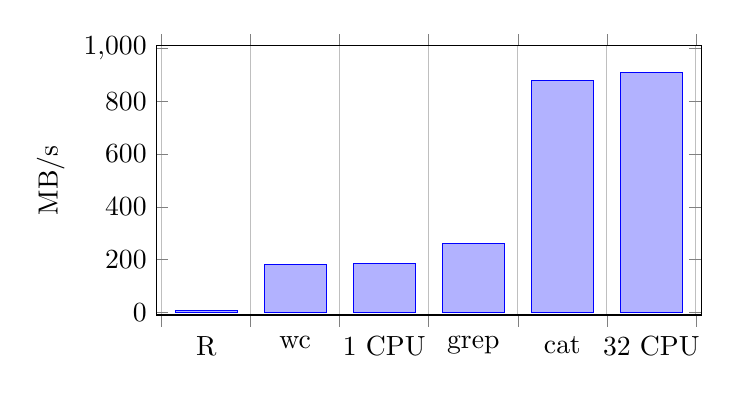
\begin{tikzpicture}
\begin{axis}[
	ylabel=MB/s,
  ymin=0, ymax=1000,
	enlargelimits=0.01,
	ybar interval=0.7,
  symbolic x coords={R, wc, 1 CPU, grep, cat, 32 CPU, end},
  width=8.5cm, height=5cm,
]
\addplot coordinates {(R,6.0) (wc,182.6) (1 CPU,186.6) (grep,261) (cat,878) (32 CPU,908) (end,0) };
% \addplot coordinates {(R,6.0) (wc,182.6) (CPU1,186.6) (grep,261) (wc -l,852) (cat,878) (Run 372,908) (Run 1,1029) (end,0) };

% \legend{MB/s}

\end{axis}
\end{tikzpicture}

\caption{Throughput comparisons of Icicle (1 CPU and 32 CPU) against existing R code and standard Unix utilities; higher is faster.}
\label{fig:bench:other}
\end{figure}



At Ambiata, we are currently using Icicle in production over medium-sized datasets that fit on a single disk.
These initial results have been very promising, and we are currently implementing distribution across multiple machines to handle datasets that are tens of terabytes compressed, and do not fit on a single disk.
Incremental computation is even more important for this distributed case, as we can avoid copying terabytes of data over the network.

We evaluated Icicle by replacing an R script which ran weekly in production.
This R script works over around three hundred gigabytes of pipe-separated values (PSV) data.
It computes twelve queries over each of the thirty-one input tables, computing 372 queries in total.

The R script for this takes fifteen hours to run and is 3,566 lines of code.
In contrast, our Icicle queries take seven minutes to run, and the dictionary describing the queries is 191 lines of code.

The table in figure~\ref{fig:bench:other} shows the throughput in megabytes per second.
We compared the throughput of several programs over the same 317GB dataset:
\begin{itemize}
\item our original R implementation (R);
\item Icicle running single-threaded (1 CPU);
\item Icicle running on multiple processors (32 CPU);
\item finding empty lines with @grep "^$"@;
\item counting characters, words and lines with @wc@;
\item reading and throwing away the results with @cat > /dev/null@.
\end{itemize}

We ran all of the Unix utilities with unicode disabled using @LANG=C LC_COLLATE@ for maximum performance.
The computer we used for most of these was an Amazon EC2 @c3.8xlarge@ with 32 CPUs, 60GB of RAM, and striped, RAIDed SSD storage.
The R code requires an @i2.8xlarge@ with 244GB of memory, but we were unable to perform our other benchmarks on such a large machine.
Icicle significantly outperformed R, and the single-threaded version was on par with @wc@, while only a little slower than @grep@.
This is despite doing conceptually more work than @wc@ and @grep@.
By using multiple processors, we were able to scale up to perform as well as @cat@, approaching the disk speed.
The R code is single threaded and would require at least 150 processors to reach similar speeds, assuming perfect scaling.
These results give us confidence that our distributed implementation will be fast as well as scalable~\cite{mcsherry2015scalability}.

We have been able to achieve such good results by generating parsing code specialised to the schema, and using data-only flattening~\cite{bergstrom2013data} as an efficient representation of structures such as arrays of sum types and tuples.
By using a query plan that is close to a functional language, we are able to apply many standard optimisations such as common subexpression elimination and dead code removal.




%!TEX root = ../Main.tex

\begin{figure}

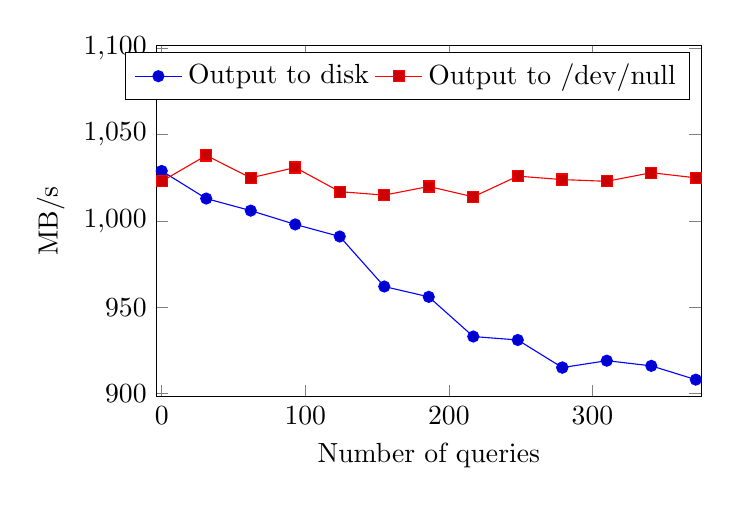
\begin{tikzpicture}
\begin{axis}[
	x tick label style={/pgf/number format/1000 sep=},
	ylabel=MB/s,
  ymin=900, ymax=1100,
%  xmax=372,
  xlabel=Number of queries,
	enlargelimits=0.01,
	legend style={legend columns=-1},
  width=8.5cm, height=6.05cm,
%	legend style={at={(0.5,-0.1)},anchor=north,legend columns=-1},
%	ybar interval=0.7,
]

% bench/raw.txt
% Running with fewer queries
% \addplot coordinates {(0,1025.5) (1,1029.6) (48,978) (96,941) (144,943) (192,936) (240,904) (276,895.5) (324,881) (372,846.2) };

% bench/raw.txt
% Running with fewer queries, better distribution
% \addplot coordinates { (0,1029) (31,1013) (62,1006) (93,998) (124,991) (155,941) (186,956) (217,933) (248,931) (279,915) (279,915) (310,919) (341,916) (372,908) };

%% APPLY LOPASS
\addplot coordinates { (0,1029) (31,1013) (62,1006) (93,998) (124,991) (155,962) (186,956) (217,933) (248,931) (279,915) (279,915) (310,919) (341,916) (372,908) };


% Fusion, no output
% \addplot coordinates { (0,1001) (31,1038) (62,1025) (93,1031) (124,1006) (155,1015) (186,1020) (217,997) (248,1026) (279,1024) (310,1009) (341,1038) (372,1025) };

%% APPLY LOPASS
\addplot coordinates { (0,1023) (31,1038) (62,1025) (93,1031) (124,1017) (155,1015) (186,1020) (217,1014) (248,1026) (279,1024) (310,1023) (341,1028) (372,1025) };

% No fusion, no output
% \addplot coordinates { (0,987) (31,1037) (62,1024) (93,1002) (124,1037) (155,1024) (186,1004) (217,1040) (248,1023) (279,998) (310,1018) (341,1013) (372,1003) };

\legend{Output to disk, Output to /dev/null};

\end{axis}
\end{tikzpicture}


\caption{Decrease in read throughput as queries are added, comparing writing the output to disk and writing to /dev/null.}
\label{fig:bench:queries}
\end{figure}


% \begin{figure}
% \begin{tikzpicture}
% \begin{axis}[
% 	x tick label style={/pgf/number format/1000 sep=},
% 	ylabel=MB/s,
%   ymin=0, ymax=1200,
%   xlabel=Number of threads,
% 	enlargelimits=0.01,
% 	legend style={legend columns=-1},
% ]
% \addplot coordinates { (1,163) (2,335) (3,442) (4,532) (5,578) (6,615) (7,633) (8,628) (9,631) (10,626) (11,637) (12,643) (13,658) (14,795) (15,781) (16,798) (17,840) (18,864) (19,862) (20,867) (21,847) (22,877) (23,876) (24,884) (25,862) };
% \end{axis}
% \end{tikzpicture}
% \caption{Scaling as threads are added}
% \label{fig:bench:scaling}
% \end{figure}




Figure~\ref{fig:bench:queries} shows how Icicle scales in throughput as more queries are added.
We ran two versions with each number of queries; one version writing output to disk, and the other throwing away the result to @/dev/null@ rather than spending time writing.
The graph shows the disk version decreasing roughly linearly in the number of queries, while the version ignoring the output stays constant.
This suggests that the output code is the bottleneck, which is unsurprising given the output format is text-based PSV.
The upshot of this is that the time spent computing the queries appears constant as hundreds of queries are added, which suggests that many more queries can be handled if a better output format is used.


%!TEX root = ../Main.tex
\section{Conclusion}
\label{s:Conclusion}

By designing a restricted language, we have a language which is just expressive enough to be useful, while retaining important performance guarantees.



% %!TEX root = ../Main.tex
\section{Elimination}
\label{s:Elimination}


Horizontal fusion for imperative loops is relatively easily, when the loops have the same number of iterations.
The problem with imperative loops occurs when trying to remove duplicate computations.
Firstly, the `definition' of a computation is split across multiple places: because the initial value of an accumulator and its update expression are in separate parts of the program, some analysis must be done to recover these.
For example, in the following loop, @a@ and @b@ have equivalent `update' expressions, but could denote very different computations depending on the implementation of @function@.
\begin{code}
a = 0;
b = 1;
for (...) {
  a = function(a);
  b = function(b);
}
\end{code}

Secondly, the order of statements in a loop affects the meaning: when accumulators are mutually dependent on each other, one can reorder the statements to produce a different, but still valid program.
These two loops are not equivalent:
\begin{code}
a = 0;
b = 1;
for (...) {
  a = a + b;
  b = a - b;
}
for (...) {
  b = a - b;
  a = a + b;
}
\end{code}

Neither of these problems are insurmountable, but the analysis required certainly complicates our goal of removing duplicate computation after fusion.

With this in mind, we will introduce our intermediate language based on what we call ``fold nests'', as opposed to loop nests.
Firstly, each accumulator should be defined in one place: this means that if two accumulators are alpha equivalent, they are equivalent.
Secondly, reordering statements (or accumulators) should not affect the meaning: two programs are equivalent if they contain equivalent sets of bindings, regardless of ordering.

We now convert the first example to folds:
\begin{code}
a = 0;
b = 1;
for (...) {
  a = function(a);
  b = function(b);
}

==>
loop ... {
  stage {
    fold a = 0
        then function(a);
  }
  stage {
    fold b = 1
        then function(b);
  }
}
\end{code}

Each fold binding must be grouped inside a @stage@ block, which allows mutual recursion across folds.
In this case, there is no mutual recursion, so the stages only contain one binding each.
The first fold is given the name @a@ with @fold a@.
Its initial value comes straight after the equals sign, so @a@ starts with a value of @0@.
The update or `kons' expression comes after @then@, and in the update expression any reference to @a@ refers to the current value of the fold.

It now becomes easier to see that the two folds are not equivalent, as the entire definitions are in one place.

The next example requires mutual recursion.
\begin{code}
a = 0;
b = 1;
for (...) {
  a = a + b;
  b = a - b;
}

==>
loop ... {
  stage {
    fold a = 0
        then a + b;
    fold b = 1
        then new a - b;
  }
}
\end{code}

Here, the update expression for @a@ refers to a later fold, @b@.
Update expressions can refer to later fold bindings in the same stage, as well as all earlier fold bindings.
The value referred to is the value of the binding at the start of the iteration, before any updates have occurred.
The new value of earlier folds, after being updated, can be referred to by suffixing a prime to the name: in the binding for @b@, the updated @a@ is referred to by @new a@.
This restriction of only accessing the new value of earlier folds is akin to the causality restriction in dataflow languages\cite{mandel2010lucy}.

Another way to think of the new value restriction above is disallowing cycles in the references to new values:
when @b@ references @new a@, the new value of @a@, it means that @new a@ must be computed before @new b@ can be.
If there were a cycle where @new a@ also depended upon @new b@, there would be no order to compute them in.
Disallowing cycles ensures an execution order.

By making the distinction between `old value' and `new value' explicit, the ordering in the program no longer has any effect on the semantics.
After converting the reordered loop with different semantics, the two programs are no longer alpha-equivalent:
\begin{code}
a = 0;
b = 1;
for (...) {
  b = a - b;
  a = a + b;
}

==>
loop ... {
  stage {
    fold b = 1
        then a - b;
    fold a = 0
        then a + new b;
  }
}
\end{code}

\subsection{Preliminary transforms}

A-normalisation is relatively easy, however any expressions in the initialiser of each fold can be lifted out as a separate fold with initialiser and an identity expression (that is, the name of the fold).
Any expressions to be lifted out from the update expression should be created as new @let@ bindings.
They cannot necessarily be created as @fold@ bindings because the expression will not work for the initial expression, if it refers to other lets or loop iterators.

Some simple forwarding can be applied, such as lets of variables, and folds where the initial and update expressions are the same.
Fold initials could be forwarded to other initials, but fold updates cannot always be forwarded to other updates, as the first evaluation of the other update will refer to the forwarder's initial.

So-called ``melting'' can be performed, splitting apart pairs into multiple bindings, arrays of pairs into pairs of arrays, and so on.
Key-value maps can be similarly split into a special map from key to index, and an array for the values.
Splitting these complex structures into their constituent parts exposes more opportunities for elimination removal.
The following program computes the mean of the loop elements. Here, the sum and count are both computed, and stored in a pair.

\begin{code}
loop item {
  stage {
    fold sumcount
     = (0, 0)
     then
       ( fst sumcount + item
       , snd sumcount + 1);

    fold mean
     = fst sumcount / snd sumcount
     then
       fst sumcount / snd sumcount;
  }
}
\end{code}

If another query were to compute the sum as well, it is not obvious looking at the two expressions that @sum@ and @fst sumcount@ are equivalent:
\begin{code}
loop item {
  stage {
    fold sum
     = 0
     then
       sum + item;
  }
}
\end{code}

Now, by splitting the @sumcount@ pair into two bindings named @sumcount1@ and @sumcount2@, it becomes easier to see that the definitions of @sum@ and @sumcount1@ are equivalent.
\begin{code}
loop item {
  stage {
    fold sumcount1
     = 0
     then
       sumcount1 + item;

    fold sumcount2
     = 0
     then
       sumcount2 + 1;

    fold mean
     = sumcount1 / sumcount2
     then
       sumcount1 / sumcount2;
  }
}
\end{code}


\subsection{Stage-local duplicate removal}
Here is an example of a stage with two counters.
\begin{code}
stage {
  fold a = 0 then c + 1
  fold b = 0 then c + 1
  fold c = 0 then a + b
}
Execution:
[ a = 0, b = 0, c = 0 ]
[ a = 1, b = 1, c = 0 ]
[ a = 1, b = 1, c = 2 ]
[ a = 3, b = 3, c = 2 ]
[ a = 3, b = 3, c = 6 ]
[ a = 7, b = 7, c = 6 ]
[ a = 7, b = 7, c = 14 ]
\end{code}

The bindings for @a@ and @b@ here are identical, and so one can be replaced with the other, by substituting @b := a@ and removing the binding for @b@.
\begin{code}
stage {
  fold a = 0 then c + 1
  fold c = 0 then a + a
}
\end{code}

Another example is a single count, spread across two recursive bindings.
Here, @a@ and @b@ depend on each other, but both have the same body modulo alpha.
\begin{code}
stage {
  fold a = 0 then b + 1
  fold b = 0 then a + 1
}
Execution:
[ a = 0, b = 0 ]
[ a = 1, b = 1 ]
[ a = 2, b = 2 ]
\end{code}

One can place them into equivalence groups based on their bodies: @a@ and @b@ go in the same equivalence group, and so any reference to @a@ or @b@ refers to the equivalence group containing both.
Equivalence groups are then squashed together, with a single binding for each equivalence group.
\begin{code}
stage {
  fold a = 0 then a + 1
}
\end{code}




\subsection{Strongly connected components}
Up to now, the reason for the stages has only been briefly mentioned.
The idea is that each stage should contain a single set of mutually recursive folds.
Then, each set of mutually recursive folds becomes a single unit to be operated on for removing duplicates.

The type system enforces that mutually recursive folds must be in the same stage, but not that each stage can only contain one set of mutually recursive folds.
We find the strongly connected components of the program graph, so that each strongly connected component.
When treating the program as a graph, each binding is a node and references to a fold @f@ as either @f@ for the current value, or @new f@ for the new value, both count as edges to @f@.

As a contrived example, we have bindings @sum@ and @count@ on their own, and another pair of bindings @a@ and @b@ which depend on each other, as well as on @sum@ and @count@.
\begin{code}
loop item {
  stage {
    fold count = 0 then count + 1;

    fold sum   = 0 then sum   + item;

    fold a     = 1 then count + b;
    fold b     = 0 then sum + new a;
  }
}
\end{code}

The graph looks something like this.
\begin{code}
  count     sum
    |        |
    V        V
    a <----> b
\end{code}

The strongly connected components are found, and ripped out into separate stages.
The bindings of each stage are sorted topologically, but this time only @new@ references count as edges in the graph.
This is because @new@ references require the new, updated value of the fold, but other references use the value that is already available at the start of the iteration.
Hence, only @new@ references impose an ordering constraint.
\begin{code}
loop item {
  stage {
    fold count = 0 then count + 1;
  }
  stage {
    fold sum   = 0 then sum   + item;
  }
  stage {
    fold a     = 1 then count + b;
    fold b     = 0 then sum + new a;
  }
}
\end{code}

\subsection{Stage layers}
Once we have a list or set of stages, we can perform a topological ordering over the stages themselves.
In this case, a whole stage becomes a node in the graph, and edges are any references between stages.

The topological ordering is used for denoting execution order between the stages, but also tells us which stages need to be checked against each other, to remove duplicates.
Each stage could be checked against all other stages, but this would be wasteful.

We can look at the topological ordering of stages as layers of the same depth.
In the @count/sum/ab@ example, @count@ and @sum@ are together on the top layer, while the stage containing @a@ and @b@ is on the second layer.

When checking for duplicates, each stage need only be compared with those on the same layer, and those on the layer directly above.
In fact, of those on the layer above, it only needs to be compared with those it refers to.
It is not necessary to check more two layers above, for example, because we know two things:
this stage refers to a binding in the layer above, while any stage two layers above cannot possibly refer to a lower stage.
However, in order to be duplicates, they must refer to the same things, or duplicates of the same things.


\subsection{Inter-stage duplicate removal}
To check if one stage is a duplicate of another, we go through each binding of the first stage, checking if there is an alpha-equivalent binding in the other stage.
We also create a substitution between the two stages.
This substitution is later performed on the rest of the program, so that after the duplicate is removed, references to the duplicate are updated to refer to the first stage.

During the process of checking, there may be multiple possible substitutions that appear to work.
The following program defines three mutually recursive counters; two of the counters increment by one, and the last increments by two.
Because of the mutual recursion, this ends up making each counter increment by a repeating pattern: one, one, two.
\begin{code}
stage {
  fold a = 0 then b + 1
  fold b = 0 then c + 1
  fold c = 0 then a + 2
}
Execution:
[ a = 0, b = 0, c = 0 ]
[ a = 1, b = 1, c = 2 ]
[ a = 2, b = 3, c = 3 ]
[ a = 4, b = 4, c = 4 ]
[ a = 5, b = 5, c = 6 ]
[ a = 6, b = 7, c = 7 ]
\end{code}

Now, suppose we wish to check if the following stage is a duplicate of the previous counters.
Note that these bindings are actually in a different order to the previous bindings, whereas the equivalent order would be @x@, @y@ then @z@.
\begin{code}
stage {
  fold y = 0 then z + 1
  fold x = 0 then y + 1
  fold z = 0 then x + 2
}
\end{code}

We start by inpsecting @y@, the first binding, and check against all bindings in the other set.
We wish to find a substitution from the names @x@, @y@ and @z@ to the names @a@, @b@ and @c@.
The substitution cannot mention any names other than those bound by the two stages.

There appear to be two possibilities for @y@: it is alpha-equivalent to both @a@ and @b@, producing two different substitutions:
\begin{code}
(Y1)
y := a
z := b
(Y2)
y := b
z := c
\end{code}

We continue checking the remaining bindings, by producing substitutions for @x@.
Like @y@, @x@ fits both @a@ and @b@, with two possible substitutions:
\begin{code}
(X1)
x := a
y := b
(X2)
x := b
z := c
\end{code}

We can cross-product these substitutions together, composing (Y1) with (X1) and so on, producing four possible substitutions.
The first two contain contradictions and are discarded immediately.
The next two seem plausible, so far.
\begin{code}
(Y1X1)
y := a
y := b
(Y1X2)
z := b
z := c
(Y2X1)
x := a
y := b
z := c
(Y2X2)
x := b
y := b
z := c
\end{code}

Now we check the final binding, @z@, which produces only one possible substitution:
\begin{code}
(Z1)
z := c
x := a
\end{code}

Composing (Z1) with (Y2X1) and (Y2X2), we find that (Y2X1Z1) is the only remaining possibility, since (Z1) and (Y2X2) are contradictory.
\begin{code}
(Y2X1Z1)
x := a
y := b
z := c
(Y2X2Z1)
x := a
x := b
\end{code}

We can now remove the stage containing @x@, @y@ and @z@, while performing this substitution over the remainder of the program, so that any references to @x@ become references to @a@, and so on.

If, for a different pair of stages, there were multiple possible substitutions after checking all bindings against the others, we could have chosen any of the substitutions.
They are all equivalent.




%!TEX root = ../Main.tex
\eject
\section{Related Work}
\label{s:Conclusion}

% This paper has introduced Icicle, a streaming query language. The streaming, single-pass nature of Icicle allows all queries over the same table to be fused into a single loop over the data.
% Icicle's modal type system allows incremental computation, ensuring that queries give the same value regardless of how the input is sliced up, and when the increments are performed.
% The modal types encode when computations are available, and disallows using the results of folds before they are finished.
% \ben{the above paragraph doesn't add any new information}.

In Icicle there is only one stream, sourced from the input table, which is implicit in the bodies of queries. This approach is intentionally simpler than existing synchronous data flow languages such as Lucy~\cite{mandel2010lucy}, as well as our prior work on flow fusion~\cite{lippmeier2013data}. Synchronous data flow languages implement Kahn networks~\cite{vrba2009kahn} that are restricted to use bounded buffering~\cite{johnston2004advances} by clock typing and causal analysis~\cite{stephens1997survey}. In such languages, stream combinators with multiple inputs, such as @zip@, are assigned types that require their stream arguments to have the same clock --- meaning that elements always arrive in lockstep and the combinators themselves do not need to perform their own buffering. In Icicle the fact that the input stream is implicit and distributed to all combinators means that we can forgo clock analysis. All queries in a program execute in lock-step on the same element at the same moment, which ensures that fusion is a simple matter of concatenating the components of the loop anatomy of each query.

Short-cut fusion techniques such as foldr/build~\cite{gill1993short} and stream fusion~\cite{coutts2007stream} rely on inlining to expose fusion opportunities. In Haskell compilers such as GHC, the decision of when to inline is made by internal compiler heuristics, which makes it difficult for the programmer to predict when fusion will occur. In this environment, array fusion is considered a ``bonus'' optimization rather than integral part of the compilation method. In contrast, for our feature generation application we really must ensure that multiple queries over the same table are fused, so we cannot rely on heuristics.

StreamIt~\cite{thies2002streamit} is an imperative streaming language which has been extended with dynamic scheduling~\cite{soule2013dynamic}. Dynamic scheduling handles data flow graphs where the transfer rate between different stream operators is not known at compile time. Dynamic scheduling is trade-off: it is required for stream operators such as grouping and filtering where the output data rate is not known statically, but using dynamic techniques for graphs with static transfer rates tends to have a performance cost. Icicle includes grouping and filtering operators where the output rates are statically unknown, however the associated language constructs require grouped and filtered data to be aggregated rather than passed as as the input to another stream operator. This allows Icicle to retain fully static scheduling, so the compiled queries consist of straight line code with no buffering.

Icicle is closely related to work in continuous and shared queries. A continuous query is one that processes input data which may have new records added or removed from it at any time. The result of the continuous query must be updated as soon as the input data changes. Shared queries are ones in which the same sub expressions occur in several individual queries over the same data, and we wish to share the results of these sub expressions among all individuals that use them. For example, in Munagala \emph{et al}~\cite{munagala2007optimization}, input records are filtered by a conjunction of predicates, and the predicates occur in multiple queries. Madden \emph{et al}~\cite{madden2002continuously} uses a predicate index to avoid recomputing them. Andrade \emph{et al} describes a compiler for queries over geospacial imagery~\cite{andrade2003efficient} that shares the results of several pre-defined aggregation functions between queries. Continuous Query Language (CQL)~\cite{arasu2002abstract,stream2003stream} again allows aggregates in its queries, but they must be builtin aggregate functions. Icicle addresses a computationally similar problem, except that our input data sets can only have new records added rather than deleted, which allows us to support general aggregations rather than just filter predicates. It is not obvious how arbitrary aggregate functions could be supported while also allowing deletion of records from the input data --- other than by recomputing the entire aggregation after each deletion.



% How to architect a query compiler~\cite{shaikhha2016architect}.
% Scheduling dynamic dataflow~\cite{buck1993scheduling}.
% Co-iterative characterization~\cite{caspi1998co}.


\section*{Acknowledgements}

\bibliographystyle{plain}
\bibliography{Main}

\end{document}


